With both MPI and CUDA independently implemented, the project can test and verify the performance scaling on various configurations. The three testable configurations are CUDA, MPI and MPI+CUDA.


\begin{figure}[!htb]
    \minipage{0.49\textwidth}
    \centering
    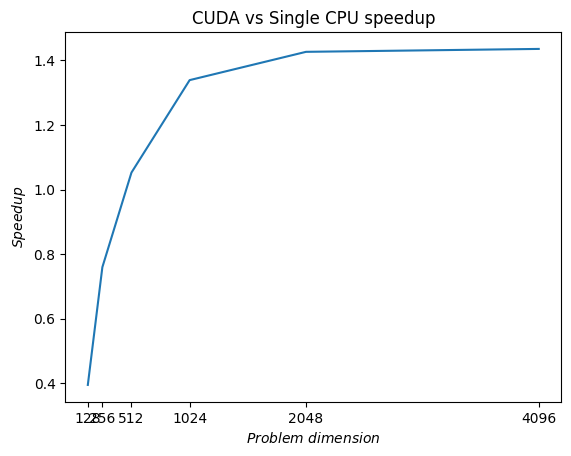
\includegraphics[height=5cm]{images/CUDA_speedup.png}
    \caption{Speedup of using CUDA on different problem sizes.}
    \endminipage\hfill
    \minipage{0.49\textwidth}
    \centering
    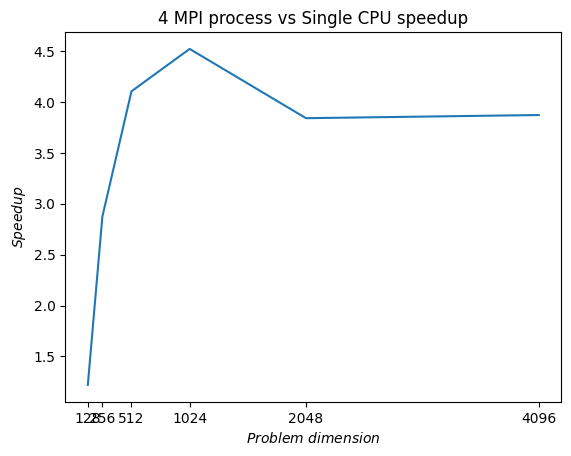
\includegraphics[height=5cm]{images/MPI_speedup.png}
    \caption{Speedup of using 4 MPI processes on different problem sizes.}
    \endminipage\hfill
    \centering
    \minipage{0.49\textwidth}
    \centering
    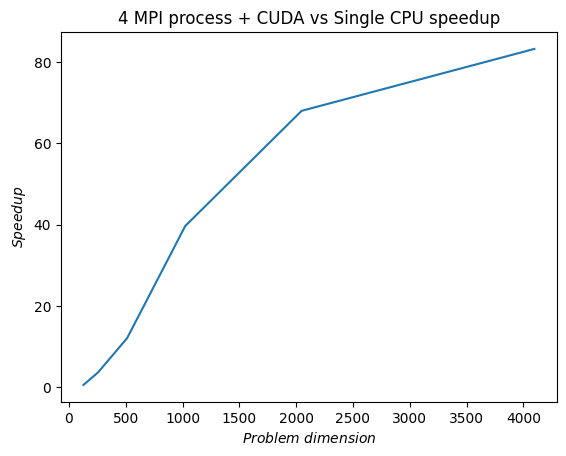
\includegraphics[height=5cm]{images/MPI_CUDA_speedup.png}
    \caption{Speedup of using 4 MPI processes with CUDA on different problem sizes.}
    \endminipage\hfill
\end{figure}

As can be seen from the graphs above, the speedup of CUDA is disappointing topping at around 42\% speedup on from the sequential version. This is a result of the overhead in initializing the GPU's global memory and the lack of locality during the propagation. Moreover, each iteration of collapse and propagation are dependent on results from the last iteration, limiting the number of warps active on the GPU to one. This is an oversight in the initial vision of this project since propagation was thought to be similar to convolution which CUDA is known to have an advantage over the CPU. The speedup managed in this implementation is mainly due to the threading and allowing all propagation to be done without looping. 

On the MPI performance, it is apparent that the overhead of collecting the final map to the CPU is significant in smaller problem sizes. Curiously, at problem size of around 1024, the performance gain is greater than the number of processes allocated for the task. This could be the result of splitting the map into sections that limited divergence and increased the rate of wave function collapse which can reduce the number of calls to the random number generator.

When combined, the speedup diminishes at 5.5 times for 4 CUDA-aware MPI processes, and shows an optimal problem size of at least 1024. 

On performance increase as the number of processors increases, the CPU-only implementation is compared against single CPU implementation, and the MPI+CUDA implementation is compared against single GPU implementation. Both are tested with a constant problem size of 2048. 

\begin{figure}[!htb]
    \minipage{0.49\textwidth}
    \centering
    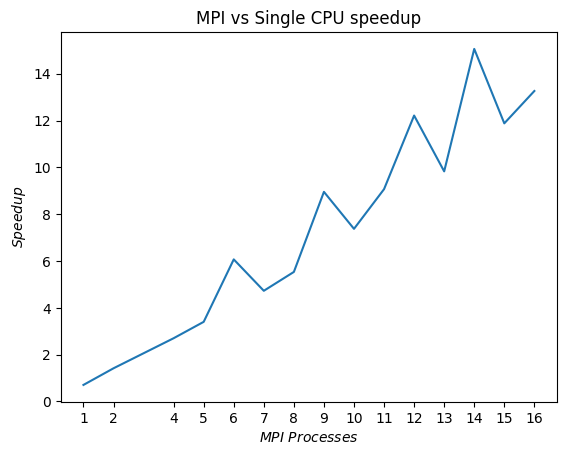
\includegraphics[height=5cm]{images/MPI_speedup_more_processes.png}
    \caption{Speedup of MPI on different number of processes.}
    \endminipage\hfill
    \minipage{0.49\textwidth}
    \centering
    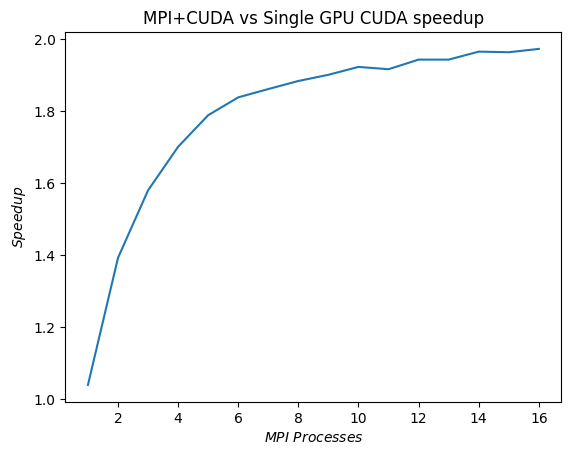
\includegraphics[height=5cm]{images/MPI_CUDA_speedup_more_processes.png}
    \caption{Speedup of MPI+CUDA on different number of processes.}
    \endminipage\hfill
    
\end{figure}

As shown above, the scaling efficiency of this MPI-oriented algorithm is high with almost linear scaling. And the CUDA-aware version shows that this the MPI communication plan can work in conjunction with other parallelization techniques. However, there exist a downward spike when allocated 11 CUDA-aware MPI processes. This could be a result of uneven problem sizes per process that causes more redundant calculation in boundary cases. 

In general, using power of twos as number of processes are favorable in terms of scaling efficiency and reducing overhead.